\documentclass[a4paper]{report}
\usepackage[utf8]{inputenc}
\usepackage[portuguese]{babel}
\usepackage{hyperref}
\usepackage{a4wide}
\hypersetup{pdftitle={TP3:  Protocolo IP},
pdfauthor={João Teixeira, José Ferreira, Miguel Solino},
colorlinks=true,
urlcolor=blue,
linkcolor=black}
\usepackage{subcaption}
\usepackage[cache=false]{minted}
\usepackage{listings}
\usepackage{booktabs}
\usepackage{multirow}
\usepackage{appendix}
\usepackage{tikz}
\usepackage{authblk}
\usepackage{bashful}
\usepackage{verbatim}
\usepackage{amsmath}
\usetikzlibrary{positioning,automata,decorations.markings}
\AfterEndEnvironment{figure}{\noindent\ignorespaces}

\begin{document}

\title{TP3:\\ 
\large Grupo Nº 7}
\author{João Teixeira (A85504) \and José Ferreira (A83683) \and Miguel Solino (A86435)}

\date{\today}

\begin{center}
    \begin{minipage}{0.75\linewidth}
        \centering
        
\includegraphics[width=0.4\textwidth]{images/eng.jpeg}\par\vspace{1cm}
        \vspace{1cm}
        \href{https://www.uminho.pt/PT}
        {\color{black}{\scshape\LARGE Universidade do Minho}} \par
        \vspace{1cm}
        \href{https://www.di.uminho.pt/}
        {\color{black}{\scshape\Large Departamento de Informática}} \par
        \maketitle
    \end{minipage}
\end{center}

\tableofcontents

\chapter{3. Captura e análise de tramas Ethernet }
\section{Exercício 1}
\textbf{Anote os endereços MAC de origem e de destino da trama capturada.}

\begin{figure}[H]
    \centering 
    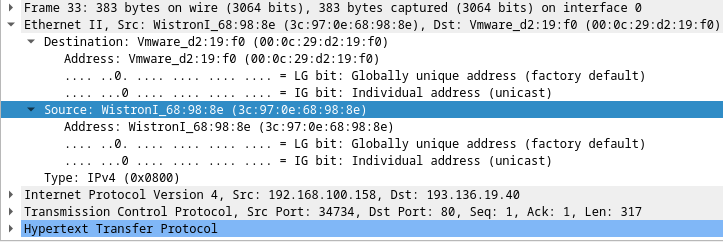
\includegraphics[width=\textwidth]{images/macAdress1.png}  
    \caption{endereço MAC}
    \label{fig:macAdress1}
\end{figure}
Observando a figura \ref{fig:macAdress1}, vemos que o endereço MAC de origem é 
3c:97:0e:68:98:8e e o destino é 00:0c:29:d2:19:f0.

\section{Exercício 2}
\textbf{Identifique a que sistemas se referem. Justifique.}
Estes dois endereços estão em dois campos diferentes, Source e Destination.
O primeiro corresponde à interface da nossa máquina nativa. O segundo
corresponde ao router da rede local à qual estamos ligados.

\section{Exercício 3}
\textbf{Qual o valor hexadecimal do campo Type da trama Ethernet? O que
significa?}

\begin{figure}[H]
    \centering 
    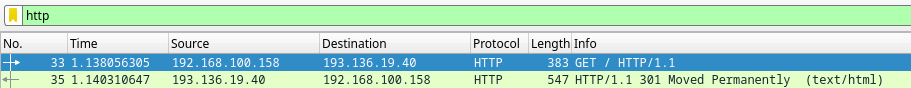
\includegraphics[width=\textwidth]{images/tramasHttp.png}  
    \caption{Tramas HTTP}
    \label{fig:tramasHttp}
\end{figure}
Como podemos observar na figura \ref{fig:tramasHttp}, no campo Type da trama
Ethernet está o valor 0x0800, que indica que o protocolo utilizado ao nível da
rede é IPv4.

\section{Exercício 4}
\textbf{Quantos bytes são usados desde o início da trama até ao caractere ASCII
“G” do método HTTP GET? Calcule e indique, em percentagem, a sobrecarga
(overhead) introduzida pela pilha protocolar no envio do HTTP GET.}

\begin{figure}[H]
    \centering 
    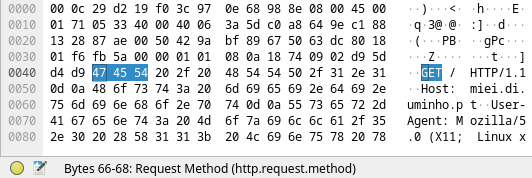
\includegraphics[width=\textwidth]{images/bytes2G.png}
    \caption{bytes até ao G}
    \label{fig:bytes2G}
\end{figure}
Observando a figura \ref{fig:bytes2G}, reparamos que até ao caractere ASCII "G"
são usados 65 bytes.
No total são utilizados 383 bytes, logo para verificar a sobrecarga fazemos o
cálculo (65/383) * 100 = 16.97%

\section{Exercício 5}
\textbf{Através de visualização direta de uma trama capturada, verifique que,
possivelmente, o campo FCS (Frame Check Sequence) usado para deteção de erros
não está a ser usado. Em sua opinião, porque será?}
Visualizando a trama reparamos que o campo FCS (Frame Check Sequence) não
aparece. Isto deve-se a estarmos a utilizar uma conexão por rede wired (neste
caso Ethernet) e este tipo é normalmente muito robusto e pouco suscetível a
erros, ao contrário das redes Wireless em que este campo já é normal aparecer.

\section{Exercício 6}
\textbf{Qual é o endereço Ethernet da fonte? A que sistema de rede corresponde?
Justifique.}

\begin{figure}[H]
    \centering 
    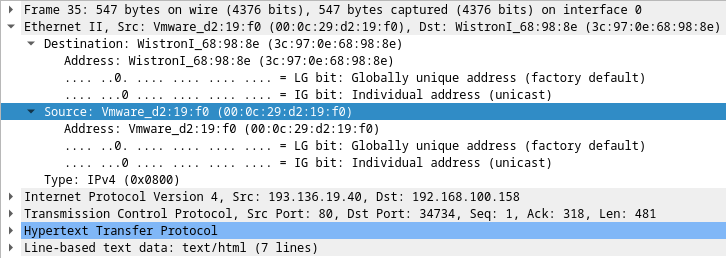
\includegraphics[width=\textwidth]{images/678.png}
    \caption{Trama Ethernet}
    \label{fig:678}
\end{figure}
Como é mostrado na figura \ref{fig:678}, o endereço Ethernet da fonte (Source) é
00:0c:29:d2:19:f0 que corresponde ao router da rede local à qual estamos
ligados.

\section{Exercício 7}
\textbf{Qual é o endereço MAC do destino? A que sistema corresponde?}
Observando outravez a figura \ref{fig:678} repara-se que o endereço Ethernet
no campo Destination é 3c:97:0e:68:98:8e e este corresponde à interface ativa da
nossa máquina nativa.

\section{Exercício 8}
\textbf{Atendendo ao conceito de desencapsulamento protocolar, identifique os
vários}
Os protocolos contidos na trama mostrada na figura \ref{fig:678} são: Ethernet
II, IPv4 (Internet Protocol Version 4), TCP (Transmission Control Protocol) e
HTTP (Hypertext Transfer Protocol).

\chapter{4. Protocolo ARP}
\section{Exercício 9}
\textbf{Observe o conteúdo da tabela ARP. Explique o significado de cada uma
das colunas.}

\begin{figure}[H]
    \centering 
    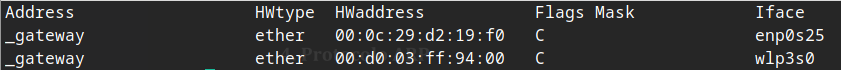
\includegraphics[width=\textwidth]{images/tabelaArp.png}
    \caption{Tabela ARP}
    \label{fig:tabelaArp}
\end{figure}
A tabela ARP pode ser assimilada a um histórico de comunicações, ou seja, mapeia
o endereço IP para o endereço MAC dos sistemas que comunicaram recentemente.
A primeira coluna representa os endereços IP, a segunda os endereços MAC e 
a terceira o tipo do endereçamento usado.

\begin{figure}[H]
    \centering 
    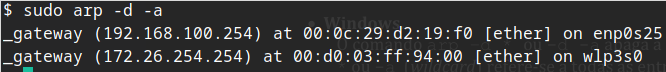
\includegraphics[width=\textwidth]{images/arpCleanup.png}
    \caption{ARP cleanup}
    \label{fig:arpCleanup}
\end{figure}

\section{Exercício 10}
\textbf{Qual é o valor hexadecimal dos endereços origem e destino na trama
Ethernet que contém a mensagem com o pedido ARP (ARP Request)? Como interpreta e
justifica o endereço destino usado?}

\begin{figure}[H]
    \centering 
    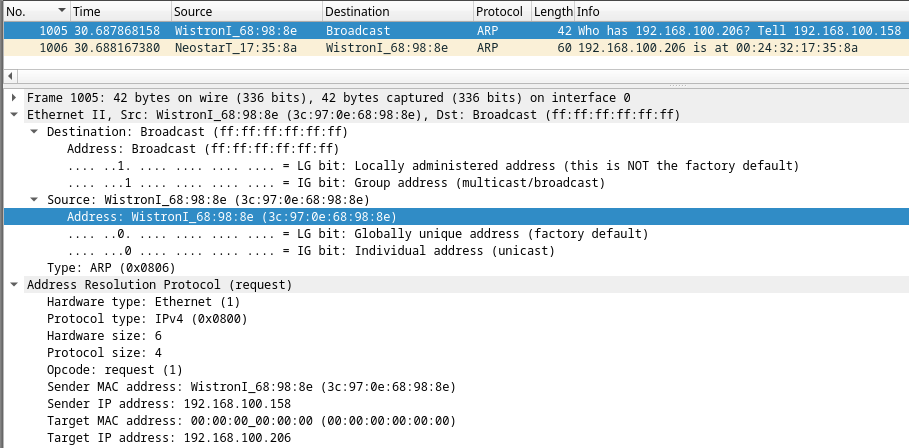
\includegraphics[width=\textwidth]{images/ex10.png}
    \caption{pedido ARP}
    \label{fig:ex10}
\end{figure}
Na trama Ethernet (figura \ref{fig:ex10}) o endereço de origem é
3c:97:0e:68:98:8e e o de destino é ff:ff:ff:ff:ff:ff. É usado este endereço de
destino para que todos os endereços conectados à rede recebam a mensagem com o
pedido.

\section{Exercício 11}
\textbf{Qual o valor hexadecimal do campo tipo da trama Ethernet? O que indica?}
Observando a figura \ref{fig:ex10}, vemos que o campo Type tem o valor 0x0806, 
indicando que o campo de dados pertence ao ARP.

\section{Exercício 12}
\textbf{Qual o valor do campo ARP opcode? O que especifica?  Se necessário,
consulte a RFC do protocolo ARP.}

\begin{figure}[H]
    \centering 
    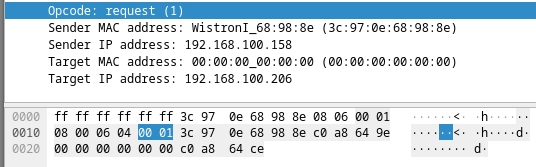
\includegraphics[width=\textwidth]{images/ex12.png}
    \caption{campo ARP opcode}
    \label{fig:ex12}
\end{figure}
Como podemos observar na figura \ref{fig:ex12}, o campo ARP opcode tem o valor
0x0001. Isso significa que o pedido é um pedido ou uma resposta, sendo neste
caso um pedido.

\section{Exercício 13}
\textbf{Identifique que tipo de endereços está contido na mensagem ARP? Que
conclui?}
A mensagem ARP contém os endereços IP de destino e de origem e sendo que se
trata de um ARP request então também só mostra o endereço MAC do endereço IP da
origem.

\section{Exercício 14}
\textbf{Explicite que tipo de pedido ou pergunta é feito pelo host de origem?}
A pergunta que é feita pela nossa máquina é "Quem tem o endereço 192.168.100.206
Diga 192.168.100.158". Logo, como resposta vamos obter o endereço MAC do
equipamento que tiver o endereço indicado na pergunta.

\section{Exercício 15}
\textbf{Localize a mensagem ARP que é a resposta ao pedido ARP efectuado.}
\textit{a. Qual o valor do campo ARP opcode? O que expecífica?}
\begin{figure}[H]
    \centering 
    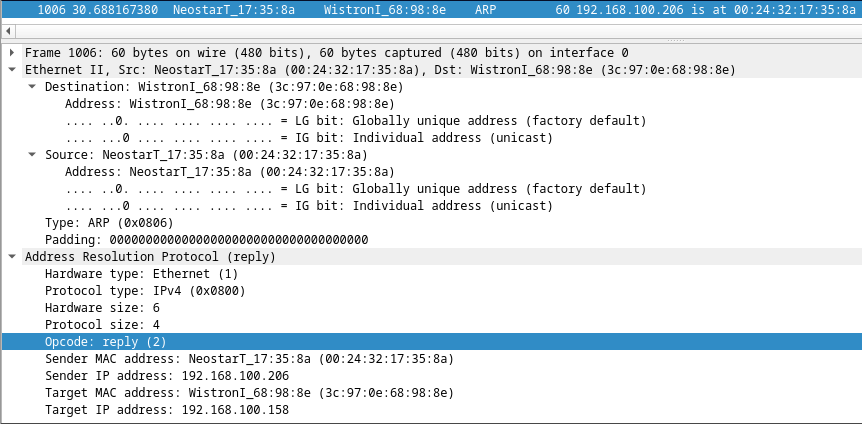
\includegraphics[width=\textwidth]{images/ex15a.png}
    \caption{campo ARP opcode}
    \label{fig:ex15a}
\end{figure}
Como podemos observar na figura \ref{fig:ex15a}, o valor do campo ARP opcode é
0x0002, o que significa que se trata de uma resposta ao pedido ARP feito
anteriormente.

\textit{b. Em que posição da mensagem ARP está a resposta ao pedido ARP?}

\begin{figure}[H]
    \centering 
    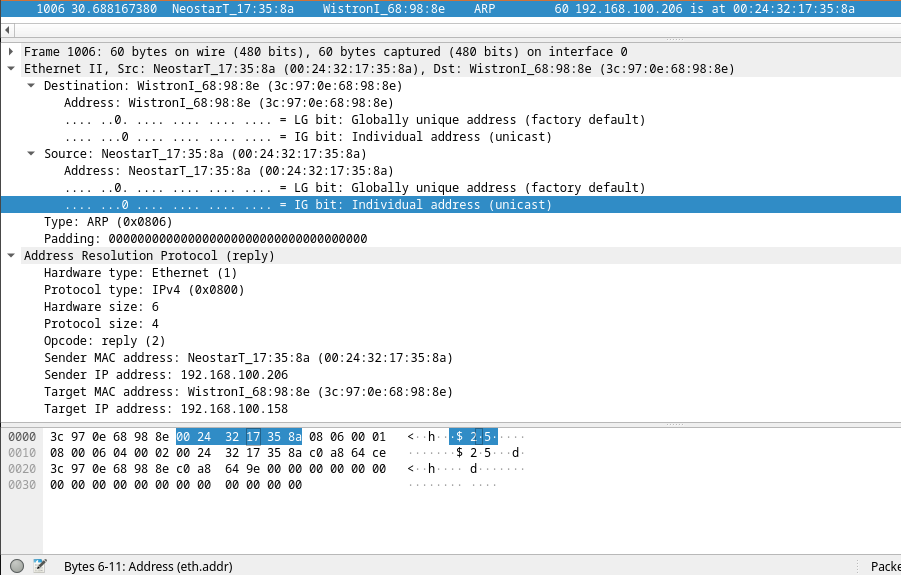
\includegraphics[width=\textwidth]{images/ex15b.png}
    \caption{pedido ARP}
    \label{fig:ex15b}
\end{figure}
Observando a figura \ref{fig:ex15b}, a resposta ao pedido ARP está entre os
bytes 6 e 11.

\section{Exercício 16}
\textbf{Identifique um pacote de pedido ARP gratuito originado pelo seu sistema.
Analise o conteúdo de um pedido ARP gratuito e identifique em que se distingue
dos restantes pedidos ARP. Registe a trama Ethernet correspondente. Qual o
resultado esperado face ao pedido ARP enviado?}

\begin{figure}[H]
    \centering 
    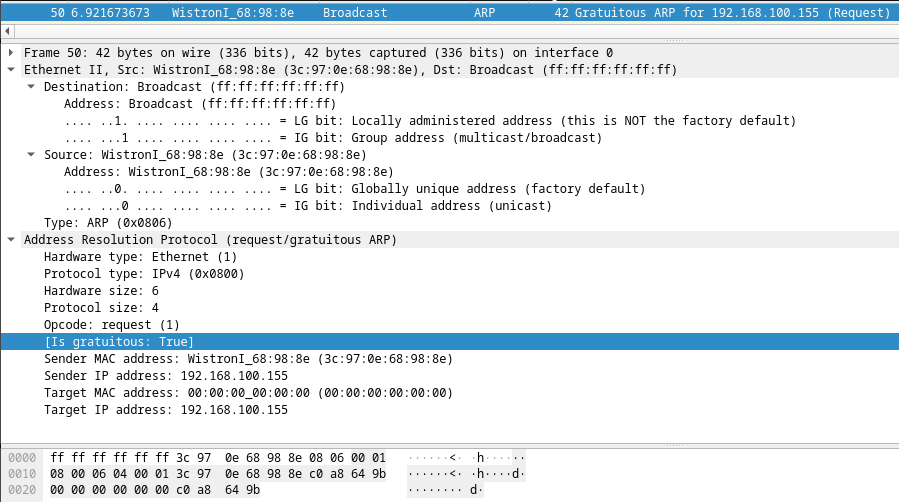
\includegraphics[width=\textwidth]{images/ex16.png}
    \caption{pacote de pedido ARP gratuito}
    \label{fig:ex16}
\end{figure}
Observando as figuras \ref{fig:ex16} e \ref{fig:ex10}, reparamos que existem
algumas diferenças. A primeira diferença é que apresenta uma flag \textit{Is
gratuitous}:True, indicando que se trata de um pedido ARP gratuito e a outra
diferença é que o Sender e Target MAC address são iguais. Ao ser um ARP gratuito
é esperado que não exista resposta, mas caso contrário acontecesse significaria
que conectado à rede existe outro equipamento com o mesmo endereço que o nosso.

\chapter{5. Domínios de colisão}
\section{Exercício 17}
\textbf{17. Faça ping de n1 para n2. Verifique com a opção tcpdump como flui o
tráfego nas diversas interfaces dos vários dispositivos. Que conclui?}
\begin{figure}[H]
    \centering 
    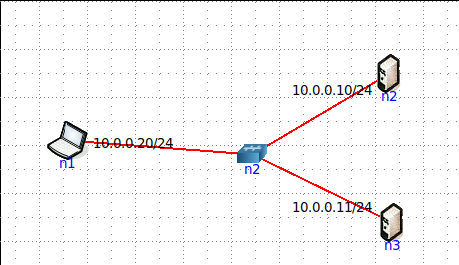
\includegraphics[width=\textwidth]{images/ex17topologiacore.png}
    \caption{Topologia Core}
    \label{fig:ex17topologiacore}
\end{figure}

\begin{figure}[H]
    \centering 
    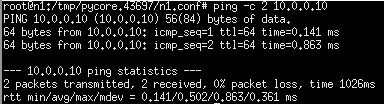
\includegraphics[width=\textwidth]{images/ex17ping.png}
    \caption{ping de n1 para n2}
    \label{fig:ex17ping}
\end{figure}

\begin{figure}[H]
    \centering 
    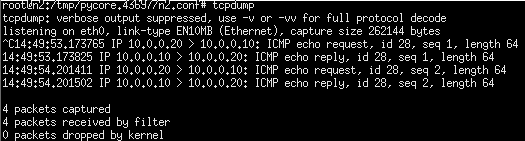
\includegraphics[width=\textwidth]{images/ex17tcpdumpn2.png}
    \caption{tcpdump em n2}
    \label{fig:ex17tcpdumpn2}
\end{figure}

\begin{figure}[H]
    \centering 
    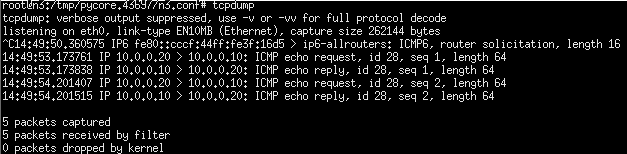
\includegraphics[width=\textwidth]{images/ex17tcpdumpn3.png}
    \caption{tcpdump em n3}
    \label{fig:ex17tcpdumpn3}
\end{figure}
Analisando as figuras \ref{fig:ex17ping}, \ref{fig:ex17tcpdumpn2} e 
\ref{fig:ex17tcpdumpn3} reparamos que os dois servidores receberam os pacotes.
Isso deve-se ao facto de o hub ao receber o ping do laptop n1 para o servidor
n2, reencaminha-os para todos os dispositivos que estejam conectados à rede.

\section{Exercício 18}
\textbf{Na topologia de rede substitua o hub por um switch. Repita os
procedimentos que realizou na pergunta anterior. Comente os resultados obtidos
quanto à utilização de hubs e switches no contexto de controlar ou dividir
domínios de colisão. Documente as suas observações e conclusões com base no
tráfego observado/capturado.}

\begin{figure}[H]
    \centering 
    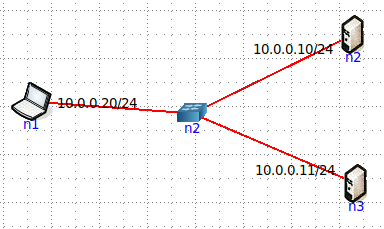
\includegraphics[width=\textwidth]{images/ex18topologiacore.png}
    \caption{Topologia Core}
    \label{fig:ex18topologiacore}
\end{figure}

\begin{figure}[H]
    \centering 
    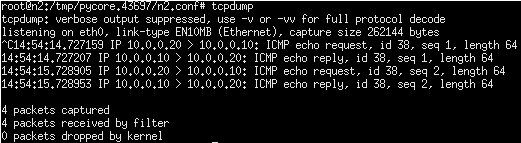
\includegraphics[width=\textwidth]{images/ex18tcpdumpn2.png}
    \caption{tcpdump em n2}
    \label{fig:ex18tcpdumpn2}
\end{figure}

\begin{figure}[H]
    \centering 
    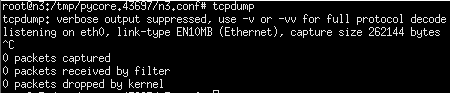
\includegraphics[width=\textwidth]{images/ex18tcpdumpn3.png}
    \caption{tcpdump em n3}
    \label{fig:ex18tcpdumpn3}
\end{figure}
Observando as figuras \ref{fig:ex18tcpdumpn2} e \ref{ex18tcpdumpn3}, reparamos
que apenas o servidor de destino do ping recebeu os pacotes. Tal acontece
porque o pedido foi enviado para um switch que envia diretamente para o host e
não envia para todos como é feito por um hub. Ou seja, ao contrário do hub, com
o switch não acontecem colisões frequentemente pois este envia para cada host as
informações usando vários canais de comunicação. Concluindo assim que os
switches são mais viáveis do que os hubs.

\chapter{Conclusão}
A realização deste trabalho proporcionou nos a oportunidade de aprofundar os
nossos conhecimentos relativamente a Ethernet, Endereços MAC, Address Resolution
Protocol (ARP) e Interligação de Redes Locais.\\
Utilizando a ferramenta Wireshark conseguimos capturar e analisar tramas
Ethernet, ou seja, o essencial para colocarmos em prática e aprimorar os nossos
conhecimentos relacionados com os tópicos anteriormente referidos.\\
Se dividirmos o trabalho por partes é possível dividir em 3. Na primeira parte o
foco foi baseado na utilização de uma conexão por Ethernet. Na segunda foi
focado nos pacotes ARP e na terceira a comparação entre Hubs e Switches.
Resumindo, achamos que maior parte do capitulo Link Layer foi abrangido e
relembrado.

\end{document}
